\subsection{Rectworld}\label[secc]{rectworld}
The Rectworld is constructed to examine the behaviour of Algorithm \ref{alg:alg1} for a larger mission space. Simulations are performed
for swarms of 3, 6 and 15 agents.

%\Crefrange{fig:3_agnt_bw_k_1_0_k_2_1_distr}{fig:3_agnt_bw_evolution}, \Crefrange{fig:6_agnt_bw_k_1_0_k_2_1_distr}{fig:6_agnt_bw_evolution}
%and \Crefrange{fig:15_agnt_bw_k_1_0_k_2_1_distr}{fig:15_agnt_bw_evolution} show the results of simulating without active dispersion ($k_{1} = 0$) for 3, 6 and 15
%agents respectively.
%
%\Crefrange{fig:3_agnt_bw_k_1_1_k_2_1_distr}{fig:3_agnt_bw_evolution_active}, \Crefrange{fig:6_agnt_bw_k_1_1_k_2_1_distr}{fig:6_agnt_bw_evolution_active}
%and \Crefrange{fig:15_agnt_bw_k_1_1_k_2_1_distr}{fig:15_agnt_bw_evolution_active} show the results of simulating with active dispersion ($k_{1} = k_{2} = 1$) for 3, 6 and 15
%agents respectively.

\begin{figure}[H]
  \centering
  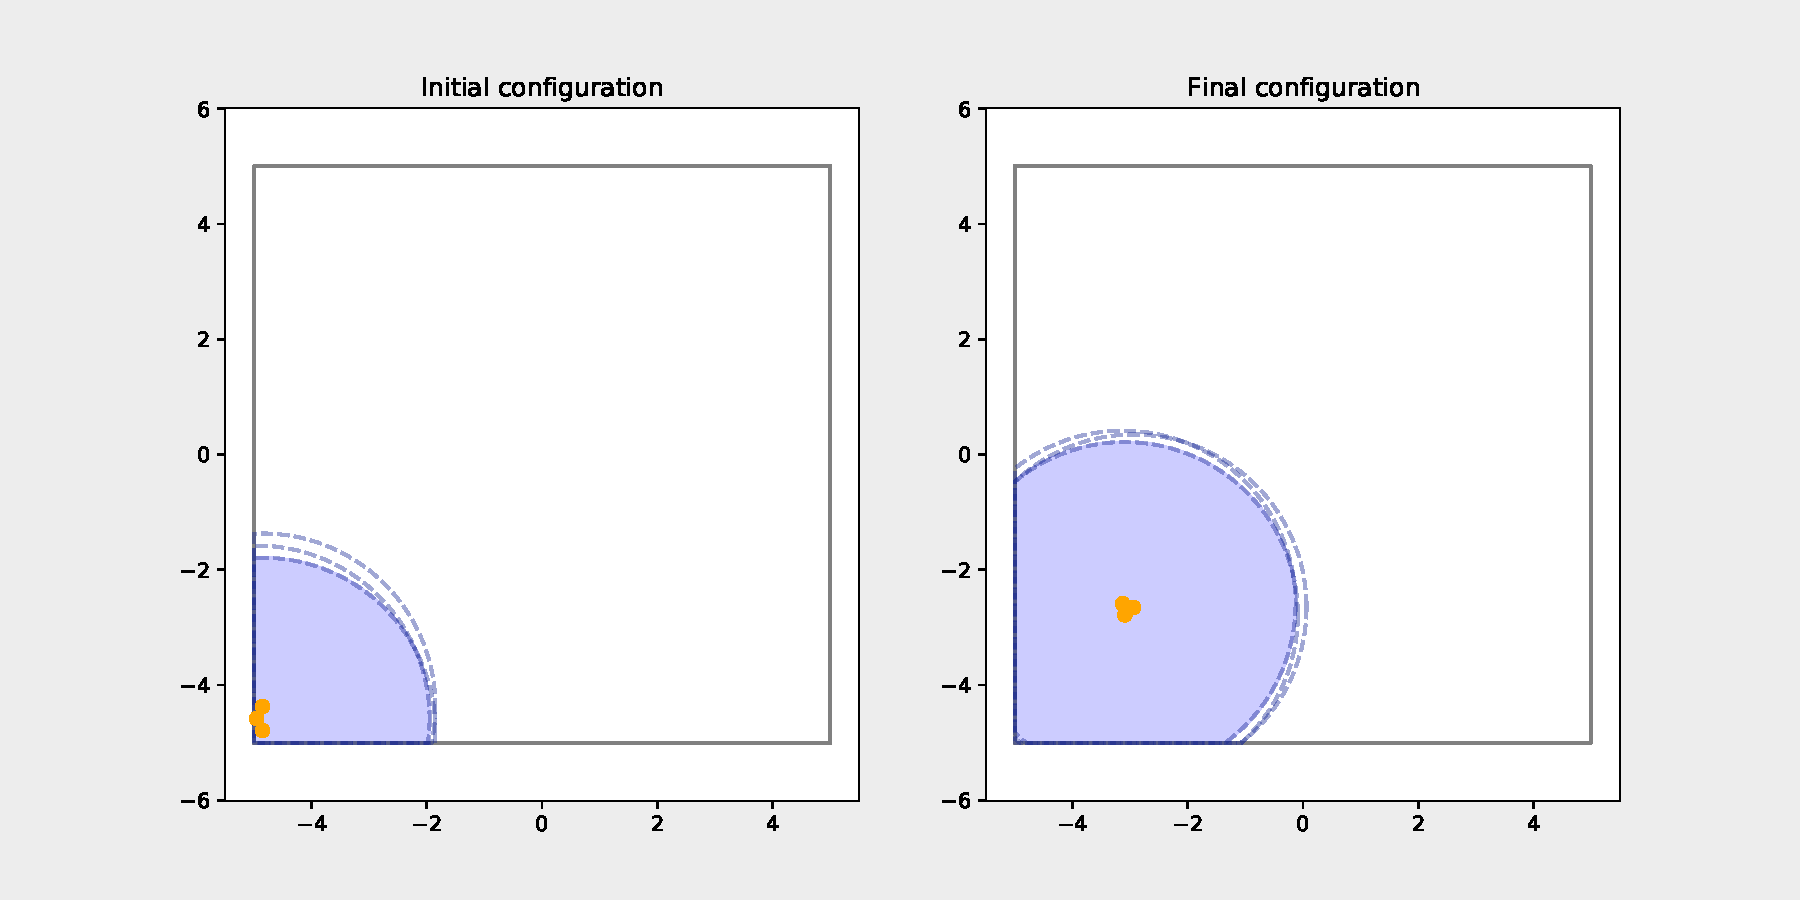
\includegraphics[width=\textwidth]{figs/bigworld_3_agnt_k_1_0_k_2_1_distr.pdf}
  \caption{Inital and final configuration of 3 agents in the Bigworld environment with $k_{1} = 0$ (no active dispersion).}
  \label{fig:3_agnt_bw_k_1_0_k_2_1_distr}
\end{figure}
\begin{figure}[H]
  \centering
  \begin{subfigure}[t]{0.5\textwidth}
    \centering
    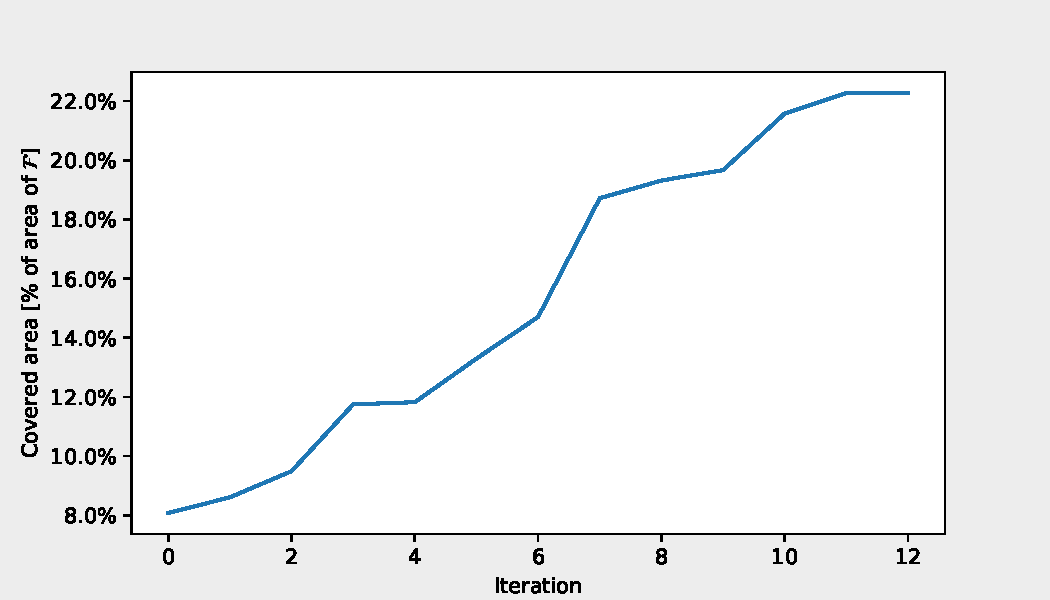
\includegraphics[width=\textwidth]{figs/bigworld_3_agnt_k_1_0_k_2_1_area_traj.pdf}
    \caption{Coverage evolution for 3 agents in the Bigworld environment with $k_{1} = 0$ (no active dispersion).}
    \label{fig:3_agnt_bw_k_1_0_a_traj}
  \end{subfigure}%
  ~ 
  \begin{subfigure}[t]{0.5\textwidth}
    \centering
    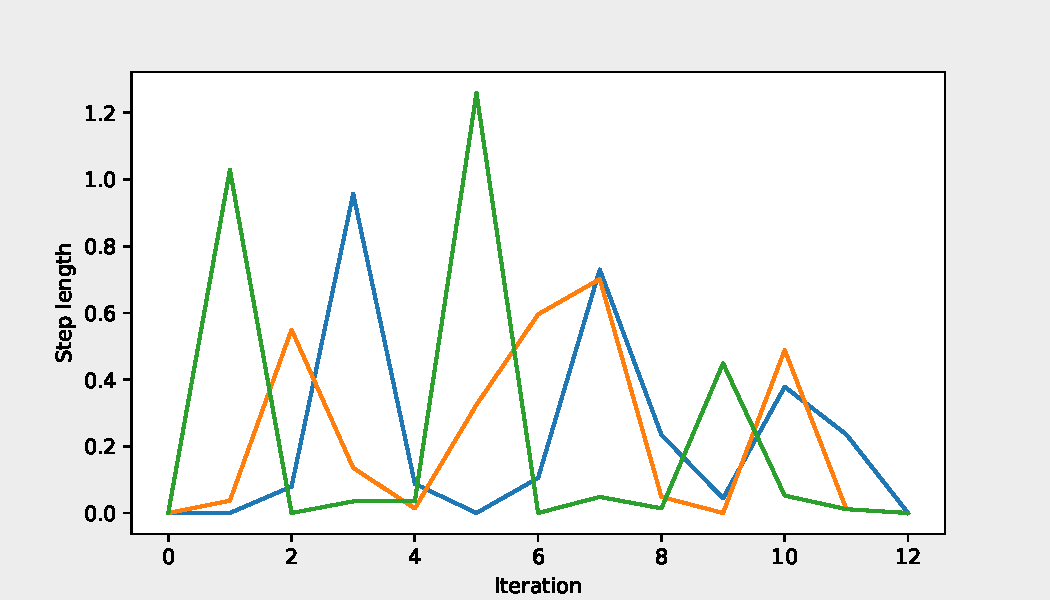
\includegraphics[width=\textwidth]{figs/bigworld_3_agnt_k_1_0_k_2_1_step_traj.pdf}
    \caption{Step length evolution for 3 agents in the Bigworld environment with $k_{1} = 0$ (no active dispersion).}
    \label{fig:3_agnt_bw_k_1_0_s_traj}
  \end{subfigure}
  \caption{Coverage percentage and step length evolution for 3 agents in the Bigworld environment when no active dispersion is used.}
  \label{fig:3_agnt_bw_evolution}
\end{figure}


\begin{figure}[H]
  \centering
  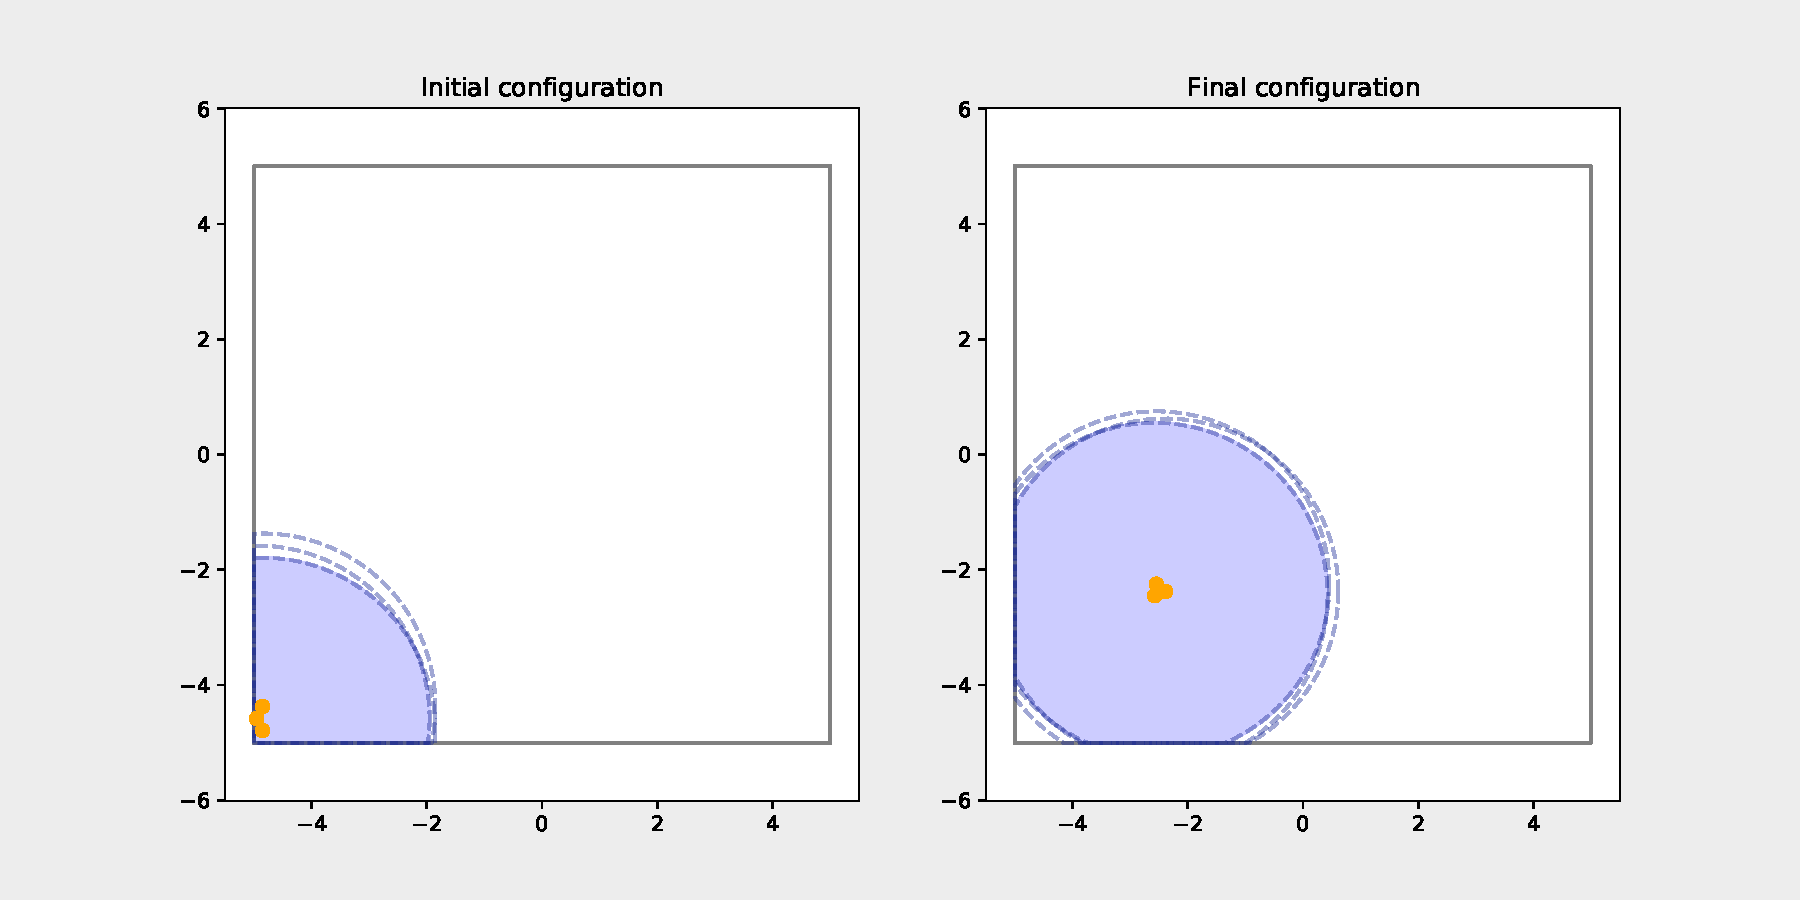
\includegraphics[width=\textwidth]{figs/bigworld_3_agnt_k_1_1_k_2_1_distr.pdf}
  \caption{Inital and final configuration of 3 agents in the Bigworld environment with $k_{1} = k_{2} = 1$ (active dispersion).}
  \label{fig:3_agnt_bw_k_1_1_k_2_1_distr}
\end{figure}
\begin{figure}[H]
  \centering
  \begin{subfigure}[t]{0.5\textwidth}
    \centering
    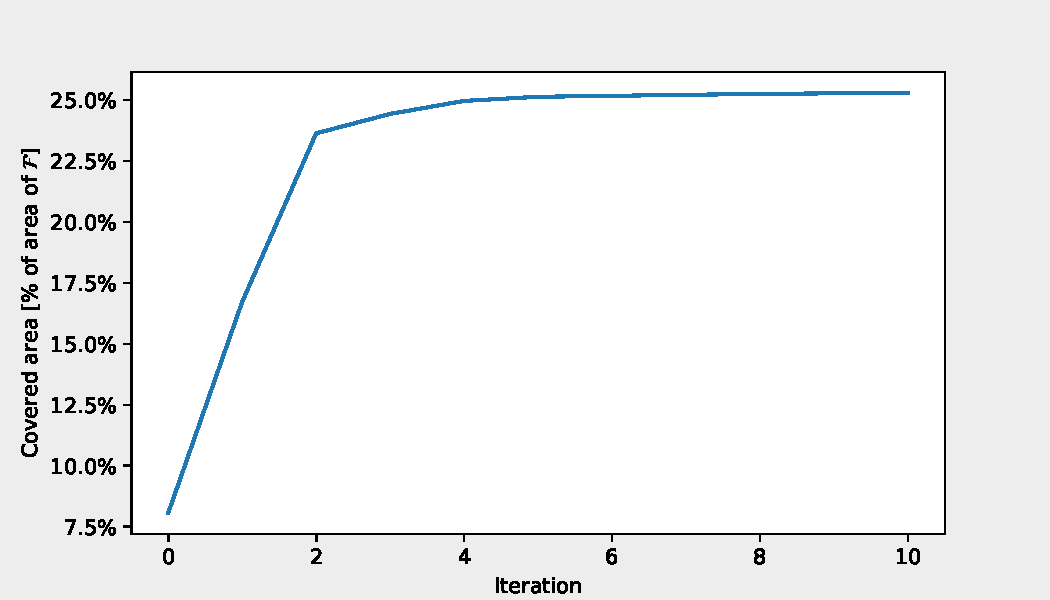
\includegraphics[width=\textwidth]{figs/bigworld_3_agnt_k_1_1_k_2_1_area_traj.pdf}
    \caption{Coverage evolution for 3 agents in the Bigworld environment with $k_{1} = k_{1} = 1$ (active dispersion).}
    \label{fig:3_agnt_bw_k_1_1_a_traj}
  \end{subfigure}%
  ~ 
  \begin{subfigure}[t]{0.5\textwidth}
    \centering
    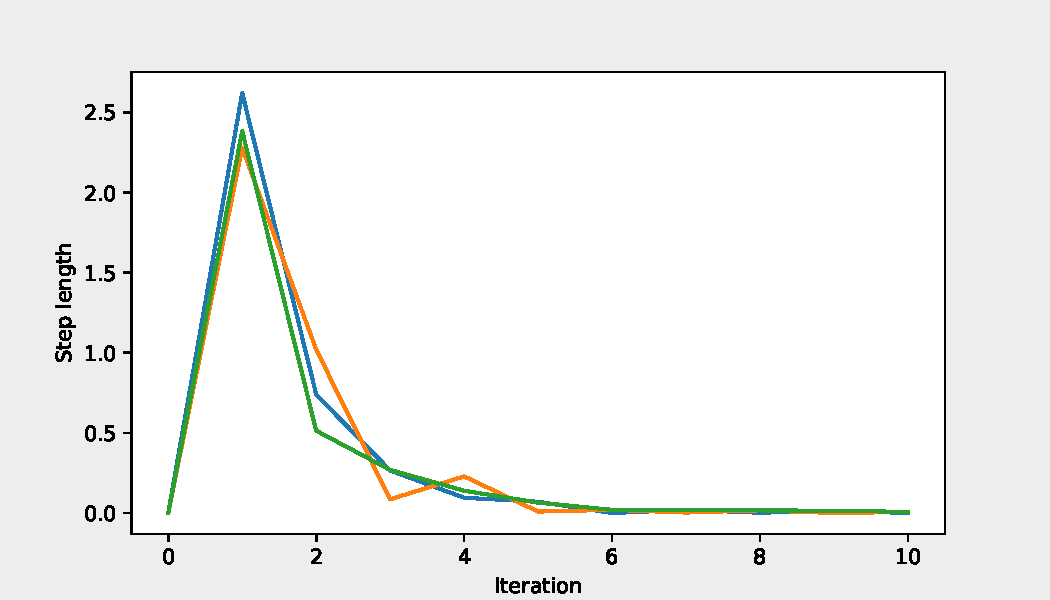
\includegraphics[width=\textwidth]{figs/bigworld_3_agnt_k_1_1_k_2_1_step_traj.pdf}
    \caption{Step length evolution for 3 agents in the Bigworld environment with $k_{1} = k_{1} = 1$ (active dispersion).}
    \label{fig:3_agnt_bw_k_1_1_s_traj}
  \end{subfigure}
  \caption{Coverage percentage and step length evolution for 3 agents in the Bigworld environment when active dispersion is used.}
  \label{fig:3_agnt_bw_evolution_active}
\end{figure}

%%%

\begin{figure}[H]
  \centering
  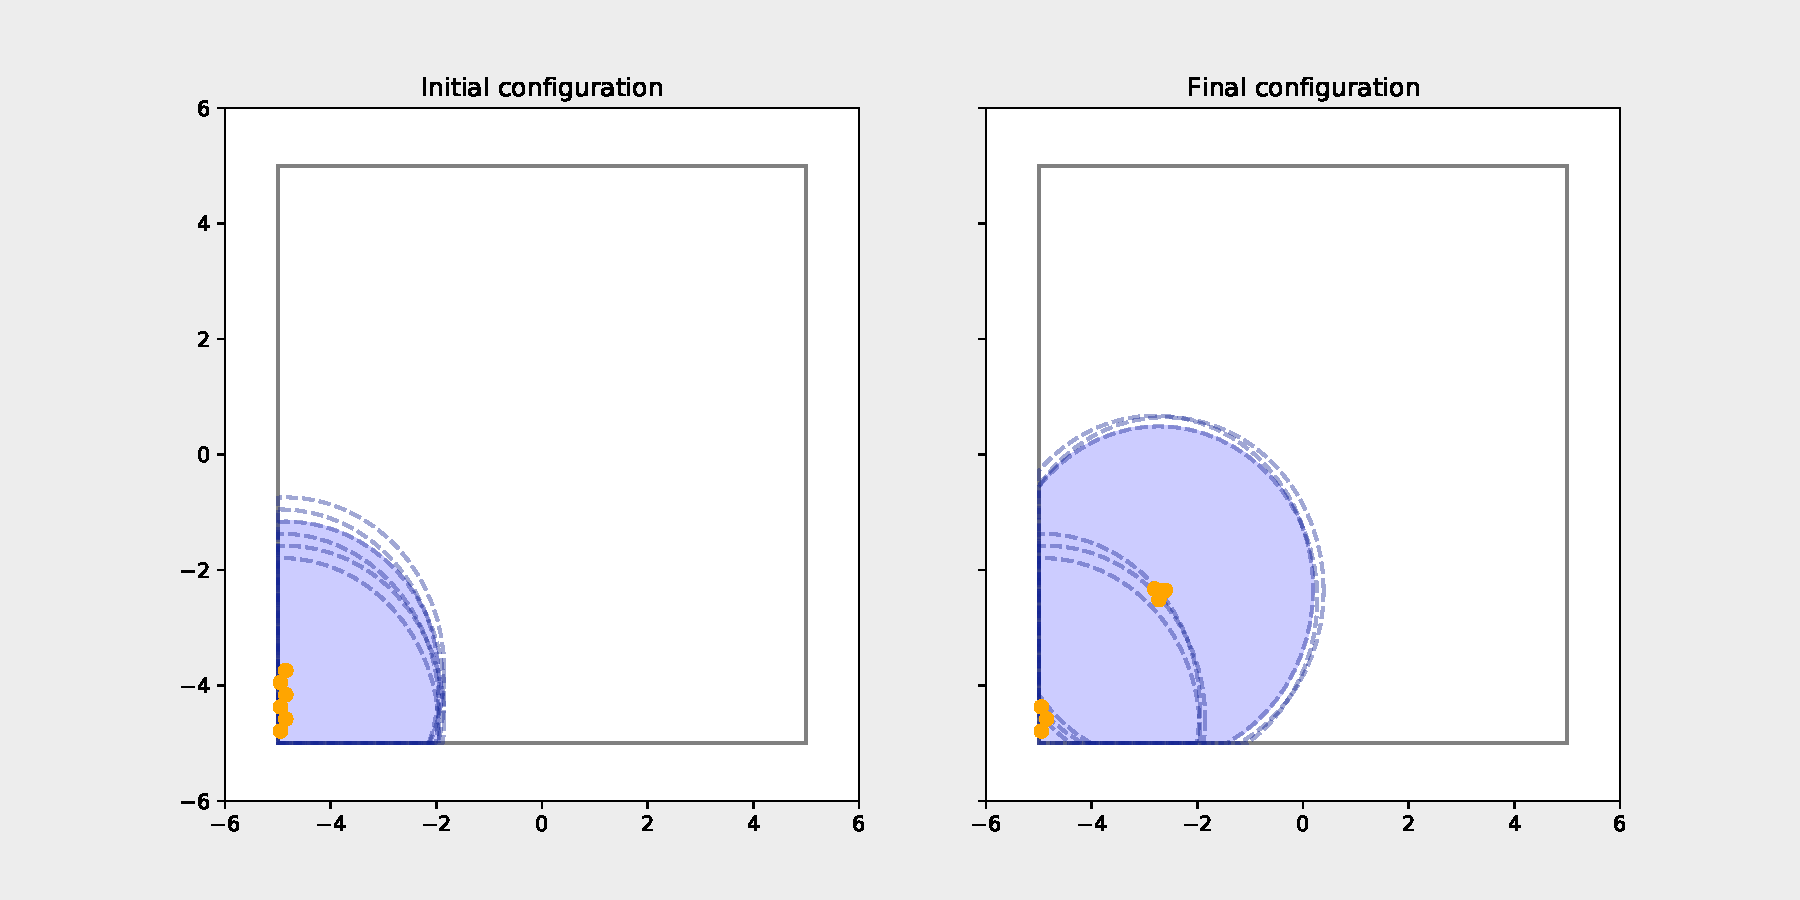
\includegraphics[width=\textwidth]{figs/bigworld_6_agnt_k_1_0_k_2_1_distr.pdf}
  \caption{Inital and final configuration of 6 agents in the Bigworld environment with $k_{1} = 0$ (no active dispersion).}
  \label{fig:6_agnt_bw_k_1_0_k_2_1_distr}
\end{figure}
\begin{figure}[H]
  \centering
  \begin{subfigure}[t]{0.5\textwidth}
    \centering
    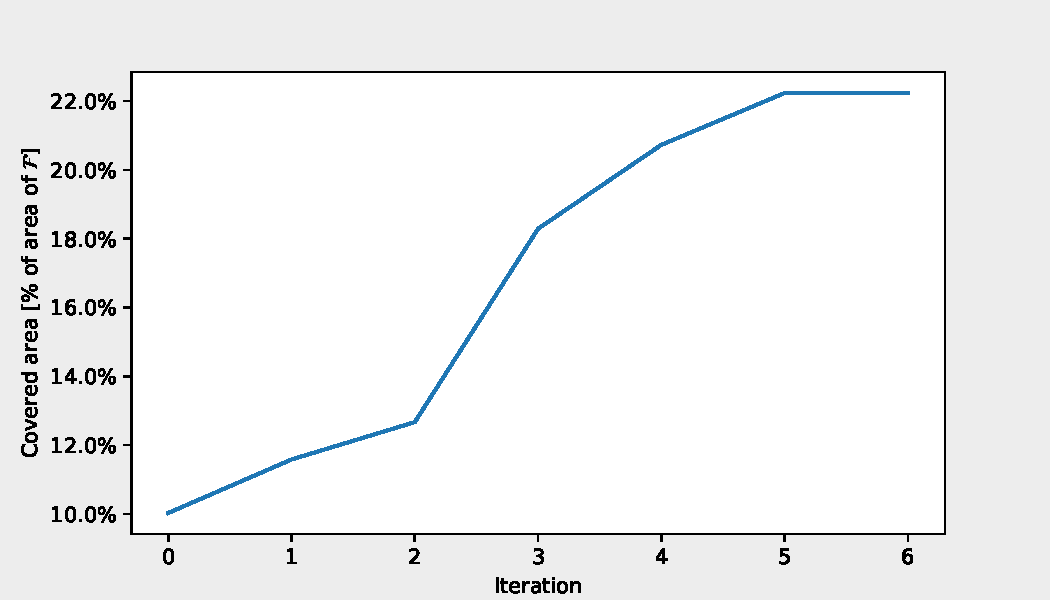
\includegraphics[width=\textwidth]{figs/bigworld_6_agnt_k_1_0_k_2_1_area_traj.pdf}
    \caption{Coverage evolution for 6 agents in the Bigworld environment with $k_{1} = 0$ (no active dispersion).}
    \label{fig:6_agnt_bw_k_1_0_a_traj}
  \end{subfigure}%
  ~ 
  \begin{subfigure}[t]{0.5\textwidth}
    \centering
    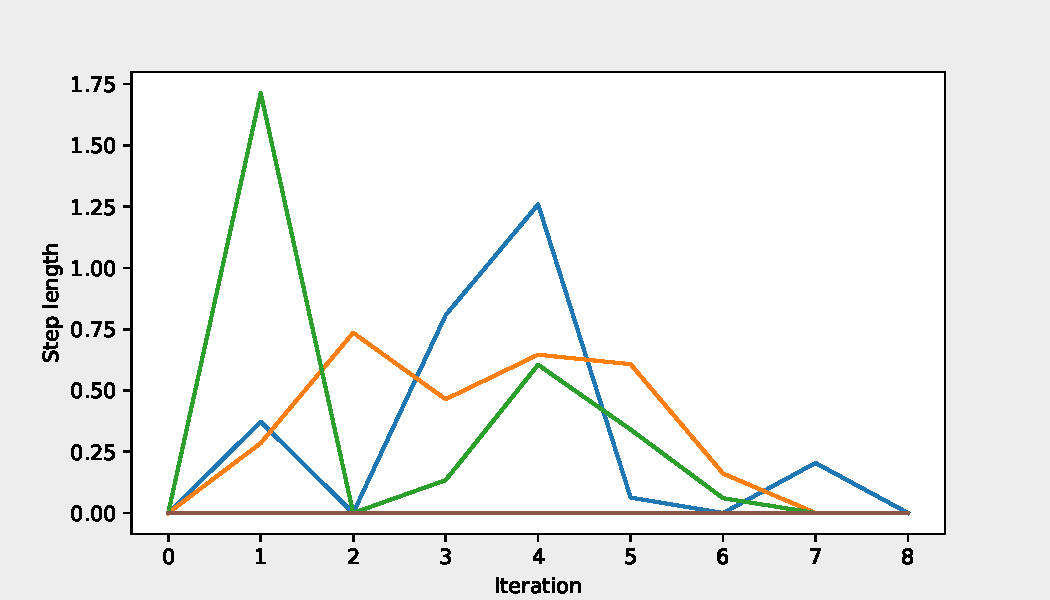
\includegraphics[width=\textwidth]{figs/bigworld_6_agnt_k_1_0_k_2_1_step_traj.pdf}
    \caption{Step length evolution for 6 agents in the Bigworld environment with $k_{1} = 0$ (no active dispersion).}
    \label{fig:6_agnt_bw_k_1_0_s_traj}
  \end{subfigure}
  \caption{Coverage percentage and step length evolution for 6 agents in the Bigworld environment when no active dispersion is used.}
  \label{fig:6_agnt_bw_evolution}
\end{figure}


\begin{figure}[H]
  \centering
  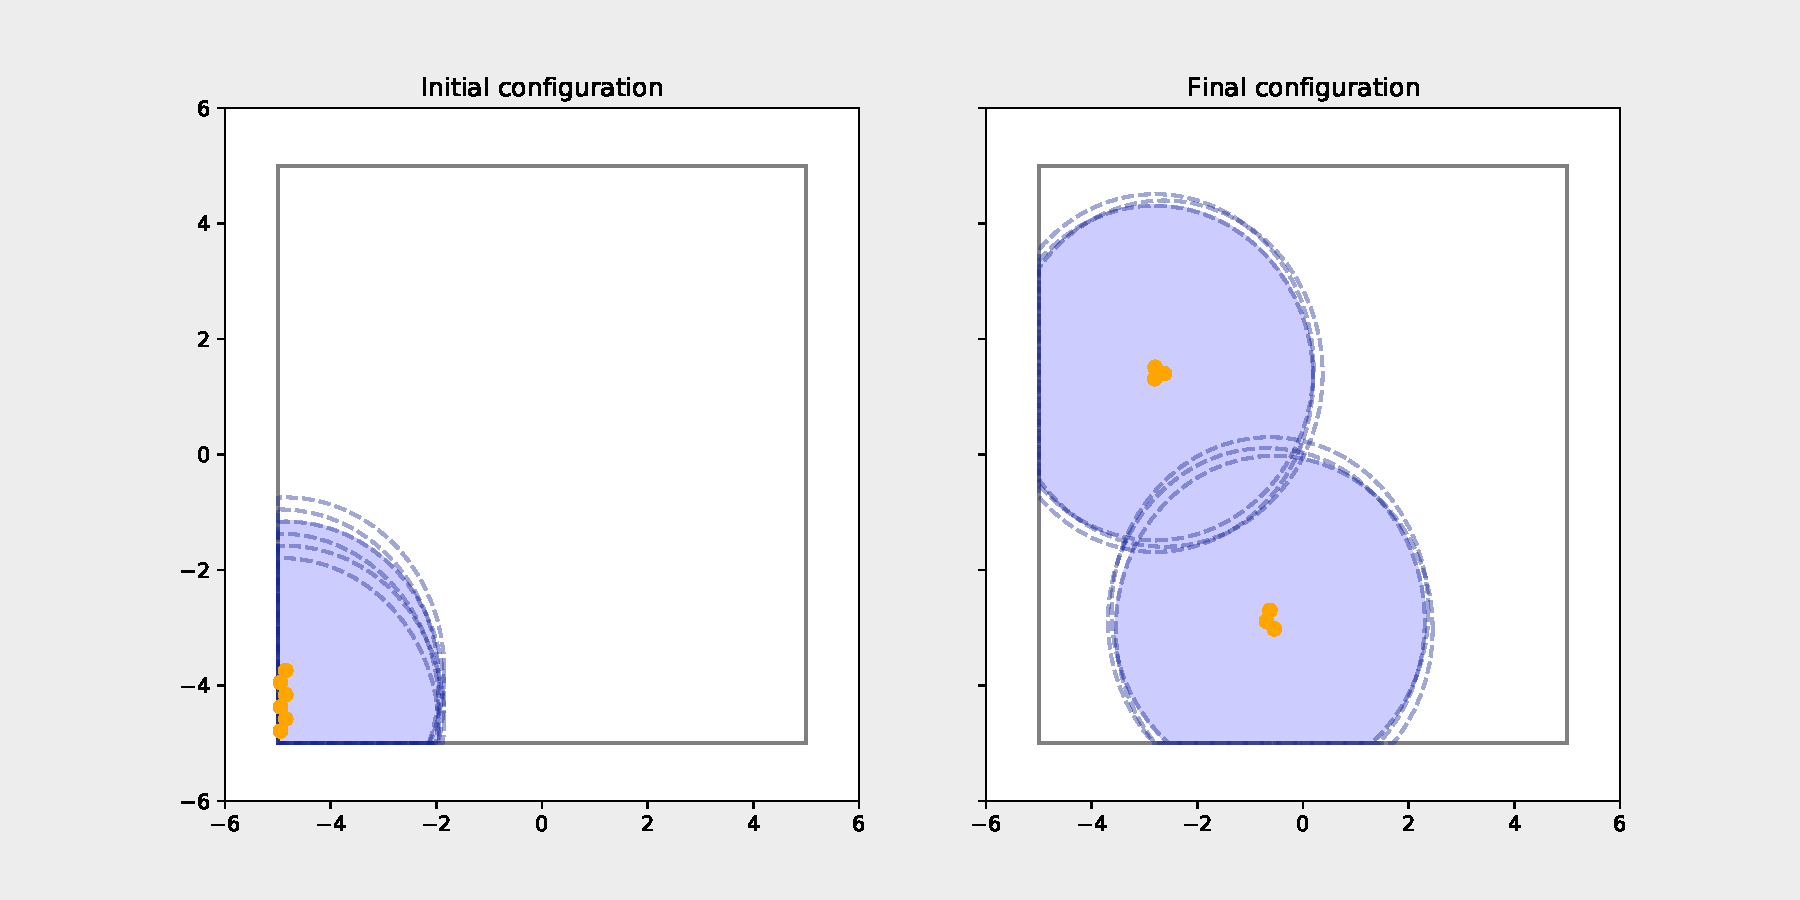
\includegraphics[width=\textwidth]{figs/bigworld_6_agnt_k_1_1_k_2_1_distr.pdf}
  \caption{Inital and final configuration of 6 agents in the Bigworld environment with $k_{1} = k_{2} = 1$ (active dispersion).}
  \label{fig:6_agnt_bw_k_1_1_k_2_1_distr}
\end{figure}
\begin{figure}[H]
  \centering
  \begin{subfigure}[t]{0.5\textwidth}
    \centering
    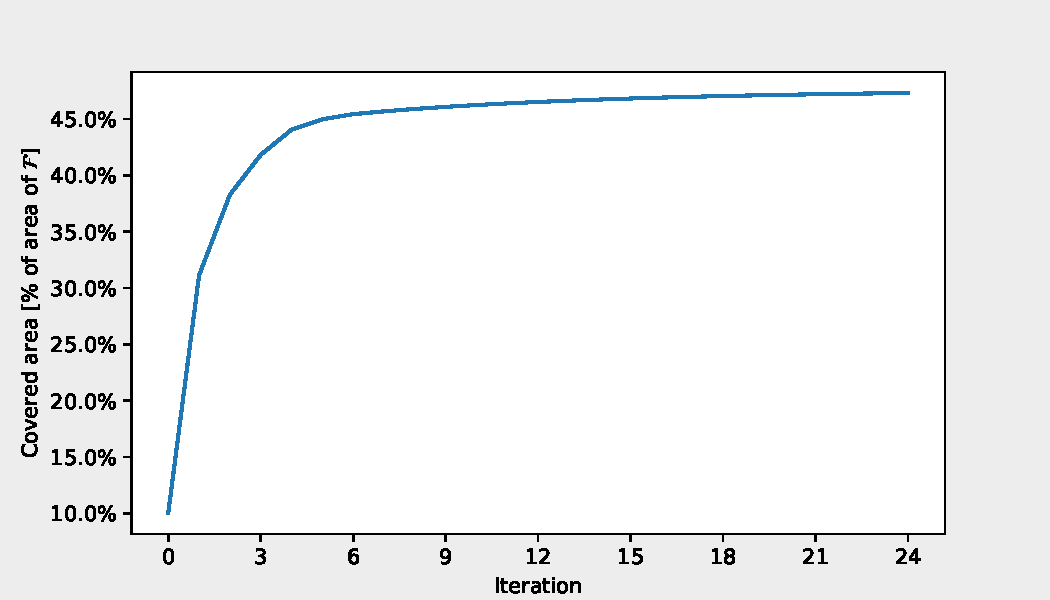
\includegraphics[width=\textwidth]{figs/bigworld_6_agnt_k_1_1_k_2_1_area_traj.pdf}
    \caption{Coverage evolution for 6 agents in the Bigworld environment with $k_{1} = k_{1} = 1$ (active dispersion).}
    \label{fig:6_agnt_bw_k_1_1_a_traj}
  \end{subfigure}%
  ~ 
  \begin{subfigure}[t]{0.5\textwidth}
    \centering
    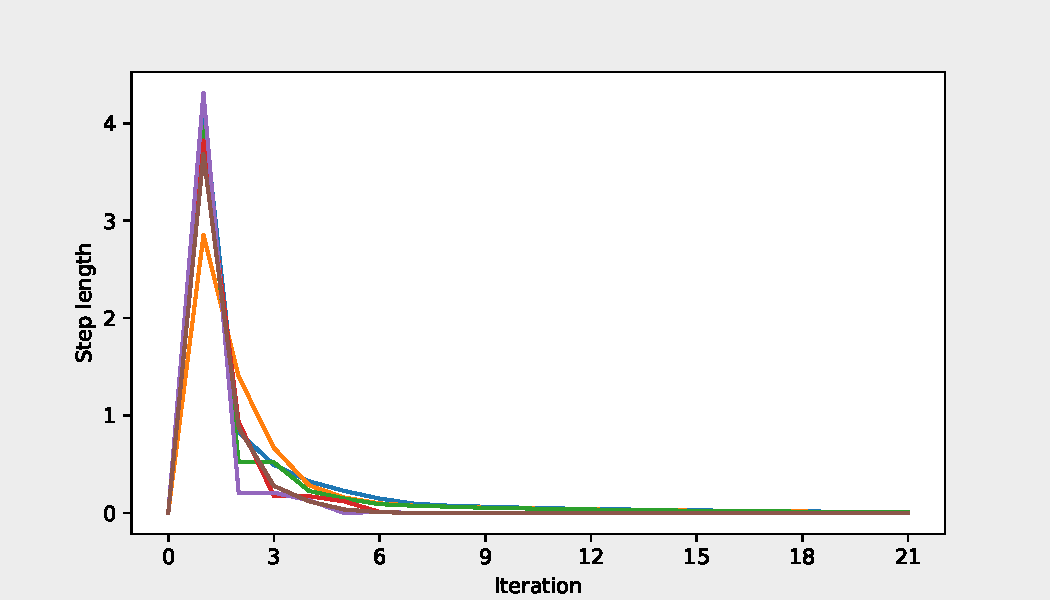
\includegraphics[width=\textwidth]{figs/bigworld_6_agnt_k_1_1_k_2_1_step_traj.pdf}
    \caption{Step length evolution for 6 agents in the Bigworld environment with $k_{1} = k_{1} = 1$ (active dispersion).}
    \label{fig:6_agnt_bw_k_1_1_s_traj}
  \end{subfigure}
  \caption{Coverage percentage and step length evolution for 6 agents in the Bigworld environment when active dispersion is used.}
  \label{fig:6_agnt_bw_evolution_active}
\end{figure}

%%%

\begin{figure}[H]
  \centering
  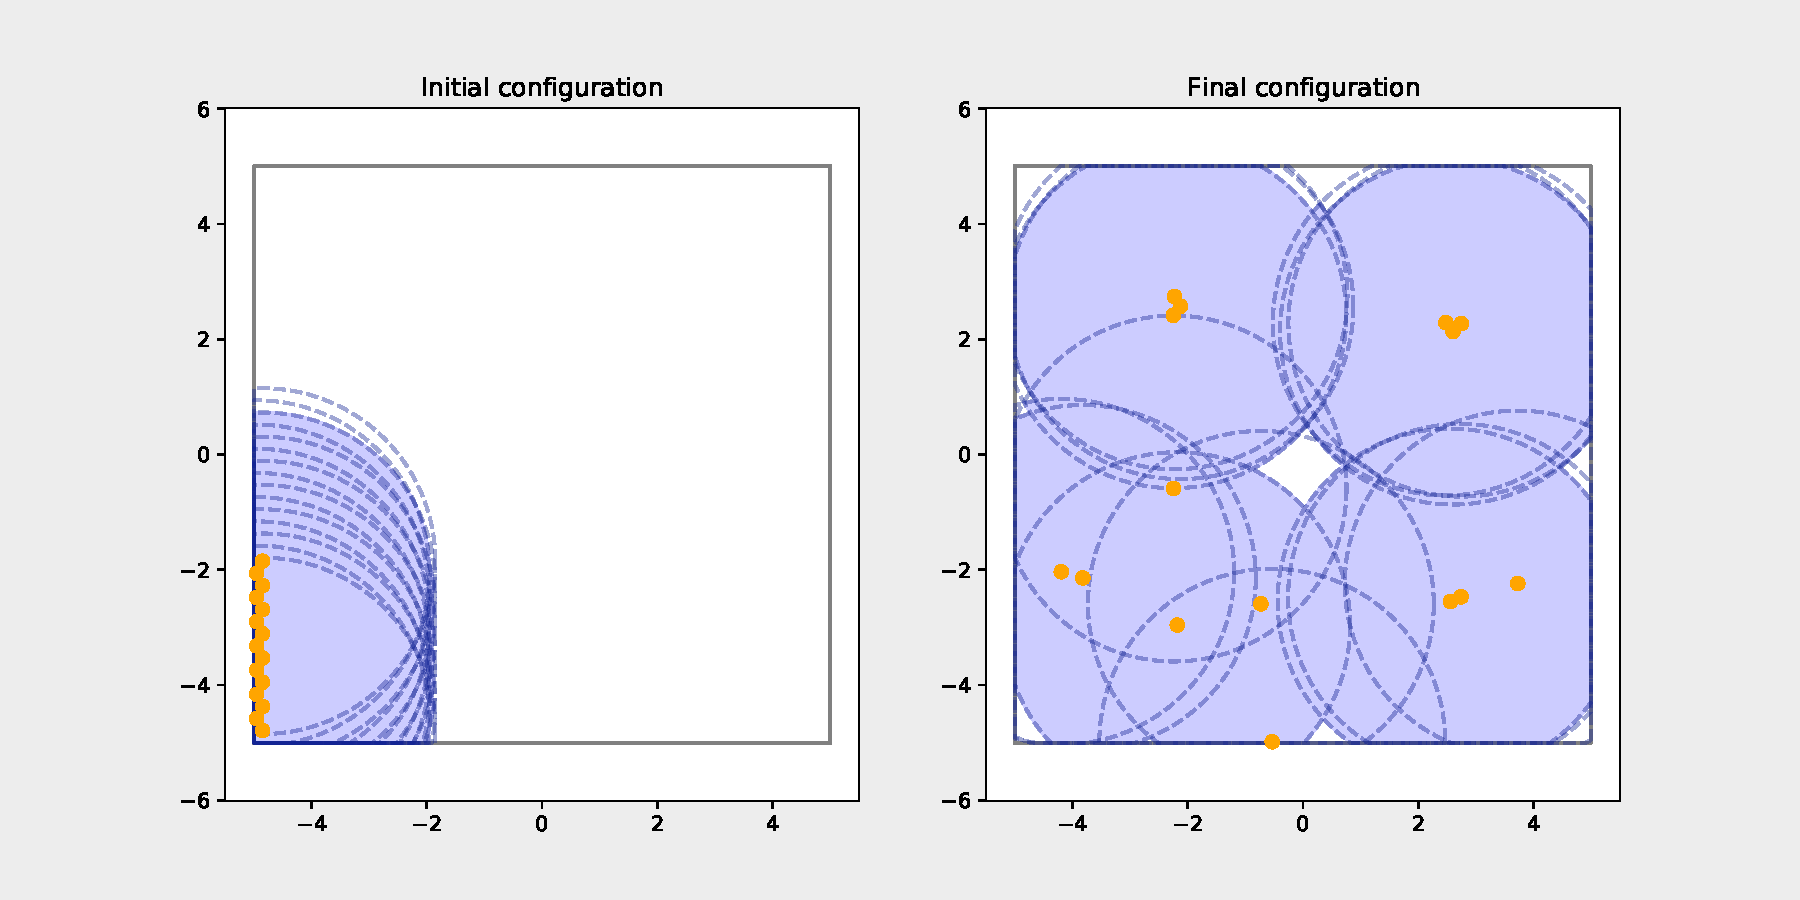
\includegraphics[width=\textwidth]{figs/bigworld_15_agnt_k_1_0_k_2_1_distr.pdf}
  \caption{Inital and final configuration of 15 agents in the Bigworld environment with $k_{1} = 0$ (no active dispersion).}
  \label{fig:15_agnt_bw_k_1_0_k_2_1_distr}
\end{figure}
\begin{figure}[H]
  \centering
  \begin{subfigure}[t]{0.5\textwidth}
    \centering
    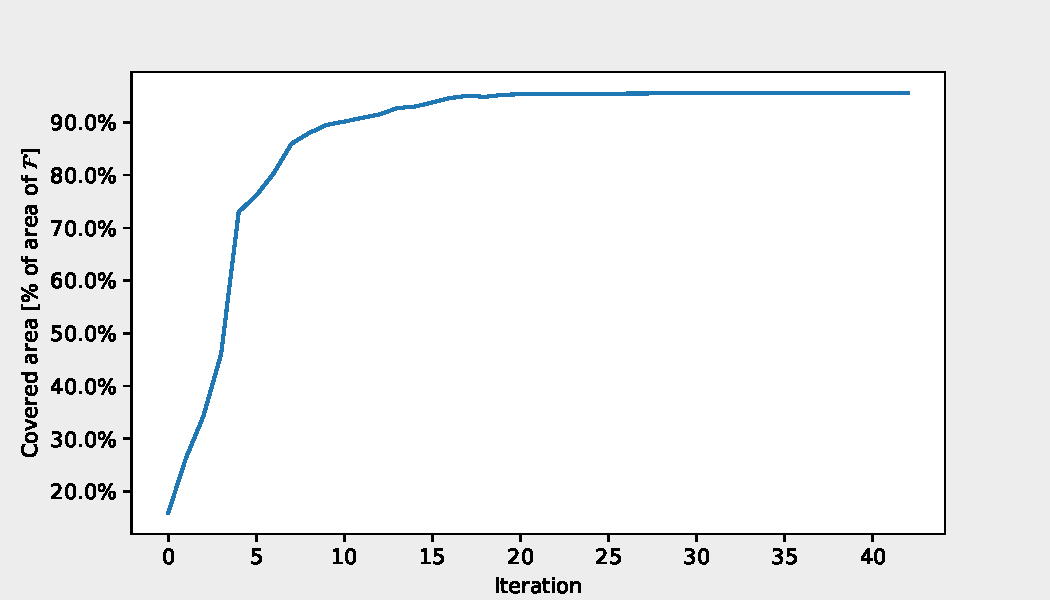
\includegraphics[width=\textwidth]{figs/bigworld_15_agnt_k_1_0_k_2_1_area_traj.pdf}
    \caption{Coverage evolution for 15 agents in the Bigworld environment with $k_{1} = 0$ (no active dispersion).}
    \label{fig:15_agnt_bw_k_1_0_a_traj}
  \end{subfigure}%
  ~ 
  \begin{subfigure}[t]{0.5\textwidth}
    \centering
    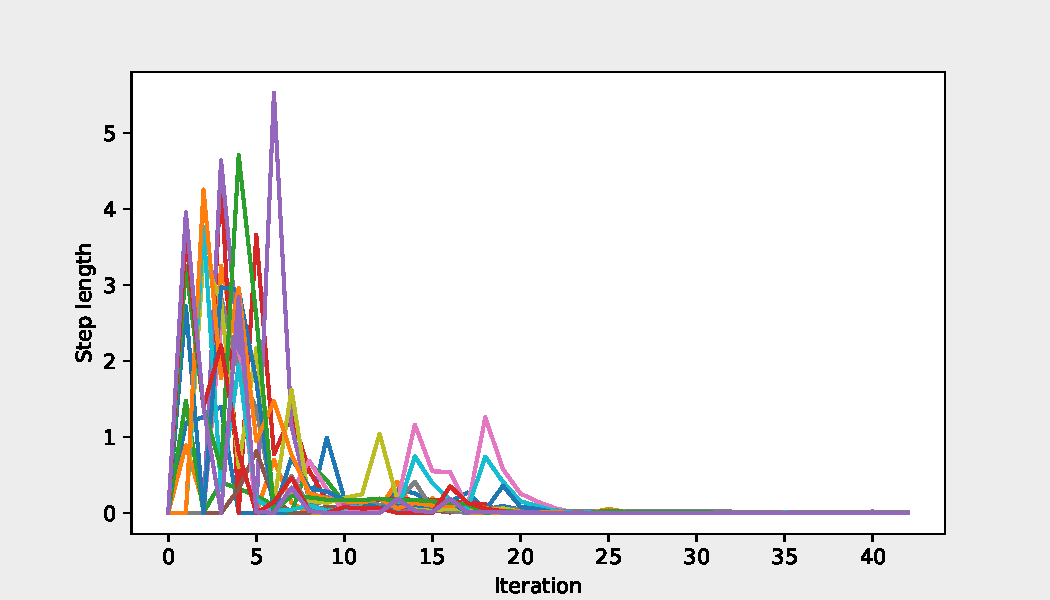
\includegraphics[width=\textwidth]{figs/bigworld_15_agnt_k_1_0_k_2_1_step_traj.pdf}
    \caption{Step length evolution for 15 agents in the Bigworld environment with $k_{1} = 0$ (no active dispersion).}
    \label{fig:15_agnt_bw_k_1_0_s_traj}
  \end{subfigure}
  \caption{Coverage percentage and step length evolution for 15 agents in the Bigworld environment when no active dispersion is used.}
  \label{fig:15_agnt_bw_evolution}
\end{figure}


\begin{figure}[H]
  \centering
  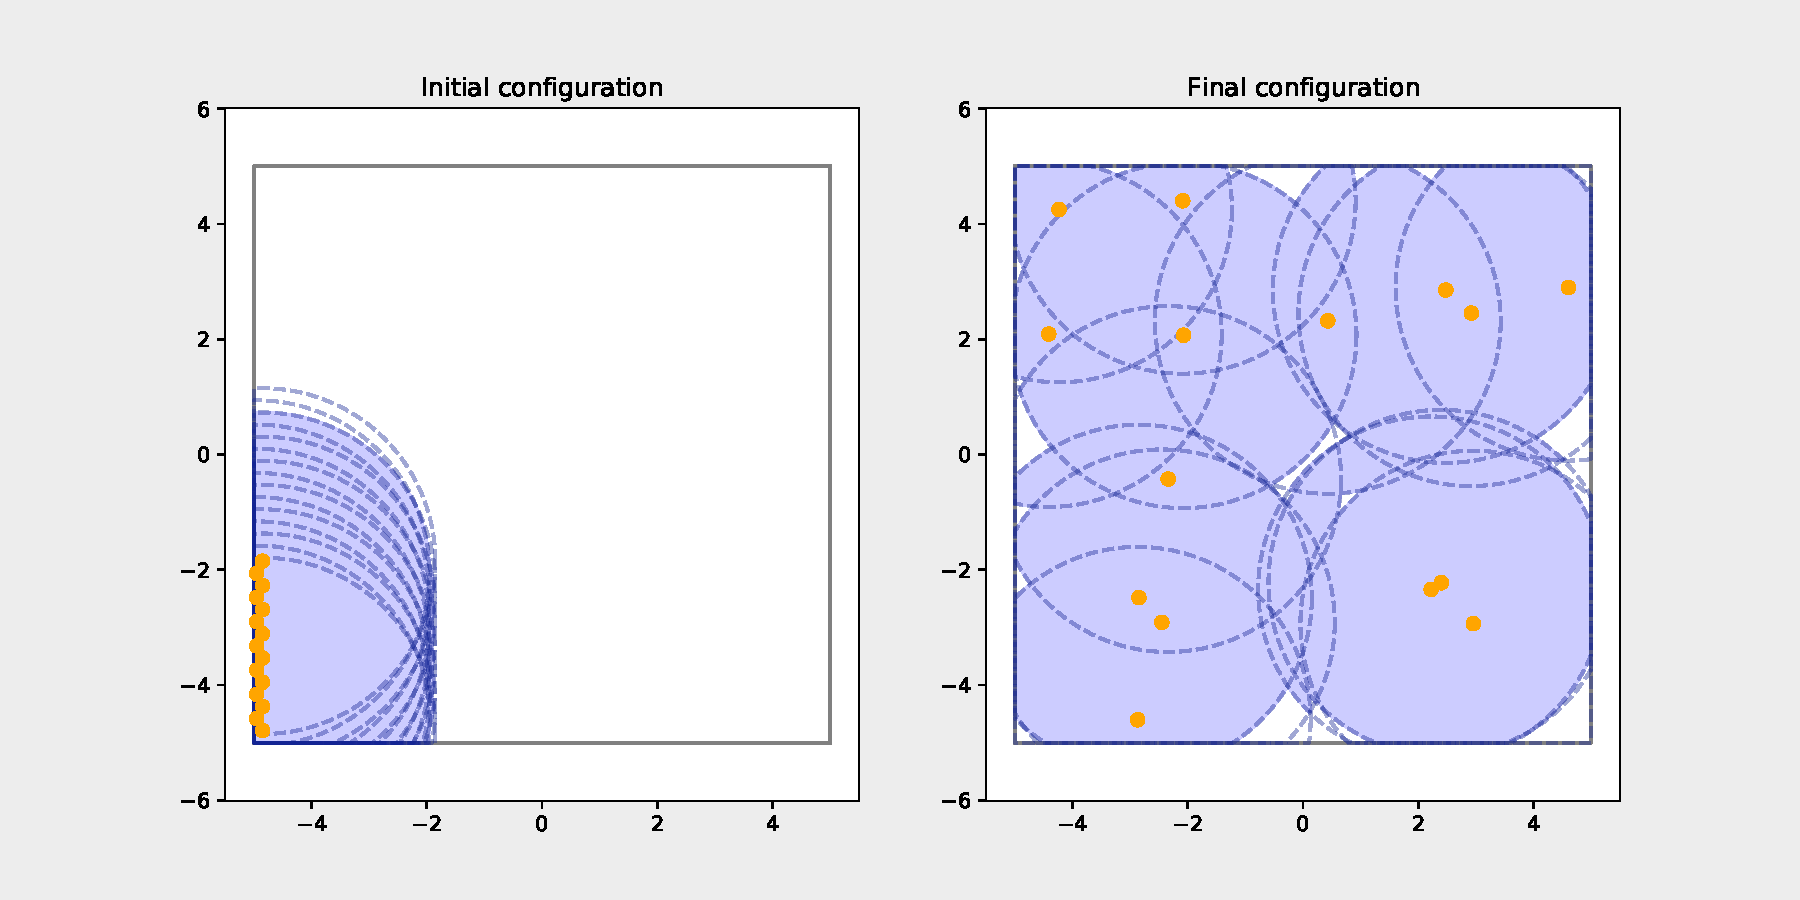
\includegraphics[width=\textwidth]{figs/bigworld_15_agnt_k_1_1_k_2_1_distr.pdf}
  \caption{Inital and final configuration of 15 agents in the Bigworld environment with $k_{1} = k_{2} = 1$ (active dispersion).}
  \label{fig:15_agnt_bw_k_1_1_k_2_1_distr}
\end{figure}
\begin{figure}[H]
  \centering
  \begin{subfigure}[t]{0.5\textwidth}
    \centering
    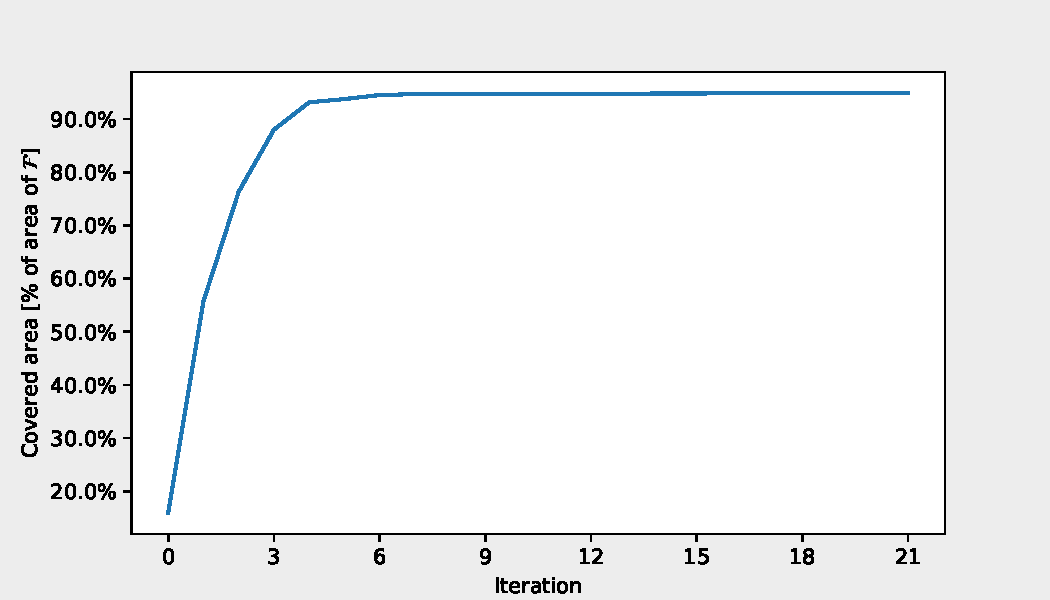
\includegraphics[width=\textwidth]{figs/bigworld_15_agnt_k_1_1_k_2_1_area_traj.pdf}
    \caption{Coverage evolution for 15 agents in the Bigworld environment with $k_{1} = k_{1} = 1$ (active dispersion).}
    \label{fig:15_agnt_bw_k_1_1_a_traj}
  \end{subfigure}%
  ~ 
  \begin{subfigure}[t]{0.5\textwidth}
    \centering
    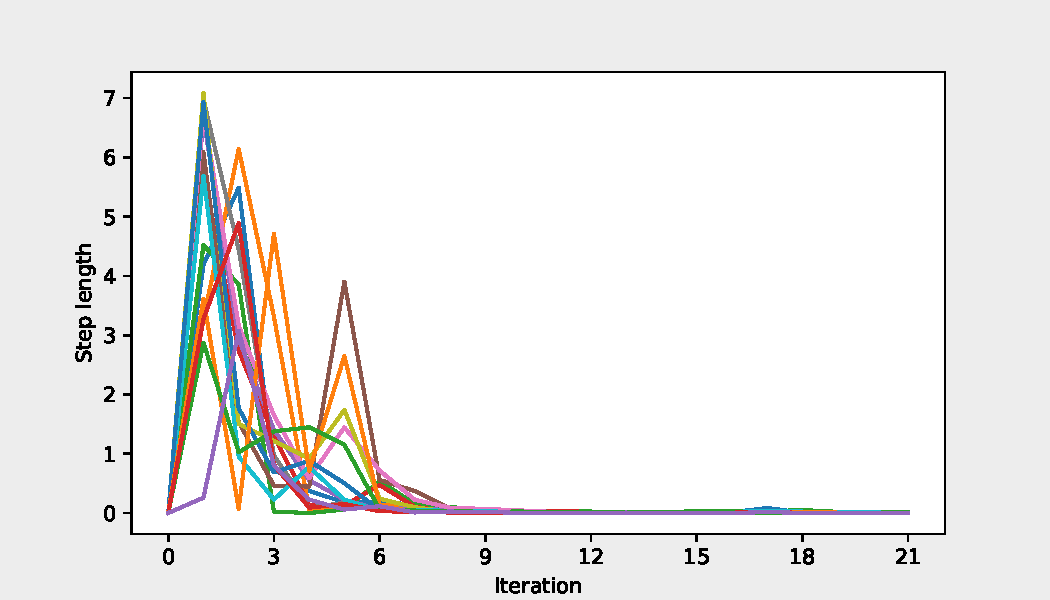
\includegraphics[width=\textwidth]{figs/bigworld_15_agnt_k_1_1_k_2_1_step_traj.pdf}
    \caption{Step length evolution for 15 agents in the Bigworld environment with $k_{1} = k_{1} = 1$ (active dispersion).}
    \label{fig:15_agnt_bw_k_1_1_s_traj}
  \end{subfigure}
  \caption{Coverage percentage and step length evolution for 15 agents in the Bigworld environment when active dispersion is used.}
  \label{fig:15_agnt_bw_evolution_active}
\end{figure}